\documentclass{article}
\usepackage[utf8]{inputenc}
\usepackage[english,ngerman]{babel}
%% ========================================================================
%%%% MISC usepackages
%% ========================================================================

%% Chemistry
\usepackage{chemfig,chemmacros}
\chemsetup{modules = all}
\chemsetup[redox]{explicit-sign = true}
\chemsetup[phases]{pos=sub}
%\chemsetup[reactions]{before-tag = {R}, tag-open = [, tag-close = ]}
  
%% Maths
\usepackage{amsmath,amssymb,amsthm,textcomp}

%% Physics
\usepackage{siunitx}

%% Graphics
\usepackage{graphicx}
\usepackage{tikz}
\usepackage{rotating}
%\usepackage{subfig}

%% Tables and Lists
\usepackage{enumerate}
\usepackage{multicol}
\usepackage{geometry}
\usepackage{tabu}
\usepackage{listings}
\usepackage{tabularx}

%% Structures and Style
\usepackage{caption}
\usepackage{subcaption}
\usepackage{booktabs}
\usepackage{colortbl}

\usepackage{xcolor}
\usepackage{xfrac}
\usepackage[export]{adjustbox}[2011/08/13]

\usepackage{booktabs}
\usepackage{float}

%% Citing and Settings
\usepackage[backend=biber,
style=numeric,
backref=true, 
natbib=true, %% offering natbib-compatible commands
hyperref=true, %% using hyperref-package references
sorting= none,
doi=true,
maxcitenames=10,
maxbibnames=100,
citestyle=numeric
]{biblatex}

\addbibresource{references.bib}

\usepackage[toc,automake]{glossaries}
\include{abbrevations}
\makeglossaries

\usepackage[colorlinks=true,linkcolor=blue]{hyperref}

%% Figure settings
\renewcommand{\figurename}{Abbildung}
\renewcommand{\tablename}{Tabelle}
\renewcommand{\listfigurename}{Abbildungsverzeichnis}
\renewcommand{\listtablename}{Tabellenverzeichnis}

%% ========================================================================
%%%% Document Information
%% ========================================================================

%% Title
\title{Darstellung eines Esters und Aufarbeitung der Bleiabfälle aus Aufgabe 3} % Title
\author{Autor: Florian \textsc{Kluibenschedl}} % Author name
\date{Bericht verfasst am: \today} % Date for the report

\begin{document}
  \renewtagform{reaction}[Rgl. ]{}{}
  
  \maketitle % Insert the title, author and date
  
  \begin{center}
    \begin{tabular}{r l}
      Versuchsdurchführung am: & 04. März 2019\\ % Date the experiment was performed
      Gruppe, Matrikelnummer: & 3, 11805747 \\
      Assistent: & Professor Smith % Instructor/supervisor
    \end{tabular}
  \end{center}


  \begin{abstract}
    
  \end{abstract}
  
  \section{Darstellung eines Esters}
   
    \subsection{Theoretische Grundlagen}
  
      \subsection{Motivation} \label{sec:Motivation}
        
        Ester stellen eine wichtige organische Stoffgruppe dar und kommen in vielen Bereichen zum Einsatz. So sind sie beispielsweise in Aromastoffen, Weichmachern oder Insektiziden enthalten \cite{EsterEigenschaften}. Der in diesem Versuch synthetisierte Essigsäurepentylester findet vor allem Verwendung als Lösungsmittel in der Lackindustrie und der Chromatographie \cite{Essigsaurepentyl}. Die Darstellung erfolgt über säurekatalysierte Veresterung von Pentan-1-ol mit Essigsäure - siehe . Als Katalysatoren eignen sich Säuren mit schwachen Nukleophilen als Anionen, weswegen in diesem Experiment Schwefelsäure verwendet wurde.
        
  \begin{reaction}
    Mg\sld{} + $\nu$ H\pch\aq -> Mg\pch[$\nu$] \aq{} + $\nu$ * 1/2 H2\gas{} \label{rec:MagnesiumWasserstoffAllgemein}
  \end{reaction}
  
  Angenommen, es sei bekannt, dass Magnesium als zweifach positiv geladenes Ion vorkommt ($\nu = 2$ in \ref{rec:MagnesiumWasserstoffAllgemein}). Damit ist die Stöchiometrie der obigen Gleichung bekannt und man kann durch Messung der entstehenden Menge an Wasserstoff auf die an der Reaktion beteiligte Stoffmenge an Magnesium schließen. Ist zudem die zu Beginn eingesetzte Masse an Magnesium bekannt, errechnet sich daraus direkt die Molmasse. Nimmt man nun umgekehrt die molare Masse des Magnesiums als bekannt an, kann auf die stöchiometrischen Faktoren und damit die Ionenladung geschlossen werden. 
  
  Beide Größen gleichzeitig zu bestimmen ist mit der beschriebenen Methode nicht möglich, wobei durch einen Blick auf das Periodensystem getrost die Annahme getroffen werden kann, dass $\nu = 2$.
  
    \subsection{Ziel des Experiments}
    
    Auf Basis der obigen Überlegungen ist das Ziel, eine möglichst exakte Bestimmung der Molmasse von Magnesium durchzuführen.
    
  \section{Experimenteller Teil}
  
    \subsection{Verwendete Materialien}
              
      \begin{table}[H]
        \centering
        \caption[Materialienliste, Quelle: Autor]{Auflistung der verwendeten Geräte und Chemikalien}
        \label{tab:Materialien}
        
        \begin{tabular}{@{}ll|ll@{}}
          \toprule
            Geräte & Hersteller & Chemikalie & Hersteller \\ \midrule
            \SI[mode=text]{600}{\milli\litre} Becherglas &  & metallisches \ch{Mg} &  \\
            \SI[mode=text,separate-uncertainty=true]{25.000(75)}{\milli\litre} Bürette &  & \SI[mode=text]{4}{M} \ch{HCl} &  \\
            \SI[mode=text,separate-uncertainty]{10.00(5)}{\milli\litre} Vollpipette &  & deionisiertes \ch{H2O} &  \\
            \SI[mode=text,separate-uncertainty]{10.0(1)}{\milli\litre} Messzylinder &  &  &  \\
            Thermometer &  &  &  \\
            Stativ mit Klammern &  &  &  \\
            \SI[mode=text]{14}{\centi\meter} Geodreieck &  &  &  \\ \bottomrule
        \end{tabular}
      \end{table}
    
    \subsection{Versuchsdurchführung} \label{sec:Versuch}
    
    \begin{figure}[h]
      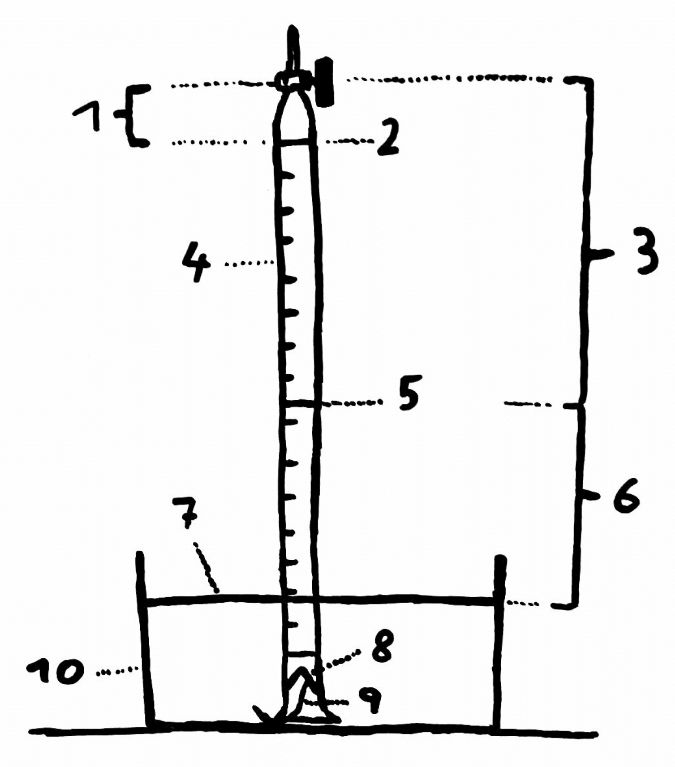
\includegraphics[scale=0.3, center]{Graphiken/Versuchsanordnungen/VersuchsanordnungMagnesium.png} 
      \caption[schematische Versuchsanordnung, Quelle: Autor]{schematische Versuchsanordnung: (1) Totvolumen, (2) \SI[mode=text]{25}{\milli\litre} Marke, (3) Gasraum - gefüllt mit \ch{H2} und \ch{H2O} Dampf, (4) Bürette - mit Klammern an einem Stativ befestigt, (5) Wasserstand in der Bürette, (6) Wassersäule, (7) Flüssigkeitsstand im Becherglas, (8) V-förmig geknichter Magnesiumstreifen, (9) Bindfaden, (10) \SI[mode=text]{600}{\milli\litre} Becherglas}
      \label{fig:Versuchsanordnung}
    \end{figure}
    
    Zu Beginn wurde das Totvolumen der Bürette bestimmt. Dazu wurde diese mit destilliertem Wasser bis zur \SI[mode=text]{25}{\milli\litre} Marke aufgefüllt und anschließend das Wasser in einen \SI[mode=text]{25}{\milli\litre} Messzylinder bis zum Hahn abgelassen. Diese Prozedur wurde 3 mal wiederholt.\\
    
    Der Versuch wurde wie in Abbildung dargestellt aufgebaut. Die Bürette wurde mit \SI[mode=text]{20}{\milli\litre} \ch{HCl} (\SI[mode=text]{4}{M}) gefüllt. Anschließend wurde mit destilliertem Wasser bis zum Bürettenrand aufgefüllt\footnote{beim Auffüllen wurde darauf geachtet, dass es zu einer möglichst geringen Aufwirbelung der Salzsäure kommt, um einem frühzeitigen Reaktionsstart vorzubeugen} und ein  Magnesiumstreifen bekannter Masse ca. \SI[mode=text]{3}{\centi\meter} in das Wasser eingetaucht. Um ein Absinken zu verhindern, hat man den Streifen V-förmig abgeknickt (um ihn zwischen den Bürettenwänden einzuklemmen) und an einem Bindfaden befestigt. Nach dem Versenken des Magnesiumstreifens wurde die Bürette bei Bedarf wieder mit destilliertem Wasser bis zum Rand aufgefüllt. 
    
    Die Reaktion wurde nun gestartet, indem die Bürette mit dem Daumen so fest wie möglich verschlossen\footnote{dabei wurde darauf geachtet, die Entstehung von Luftblasen zu vermeiden}  und verkehrt in das Becherglas getaucht wurde, wie in Abbildung gezeigt. Aufgrund der größeren Dichte von Salzsäure (\SI[mode=text]{1.19}{\gram\per\cubic\centi\metre} bei \SI[mode=text]{20}{\degreeCelsius} für eine 37 \%-ige Salzsäure \cite{Salzs}) im Vergleich zu destilliertem Wasser (\SI[mode=text]{0.997}{\gram\per\cubic\centi\metre} bei \SI[mode=text]{20}{\degreeCelsius}) diffundierte diese nach unten und reagierte mit dem Magnesiumstreifen unter Wasserstoffentwicklung. 
    
    Das Ende der Reaktion war erreicht, wenn das gesamte Magnesium reagiert hat\footnote{anzumerken ist, dass die \ch{HCl} in einem Überschuss zugegeben wurde, um eine möglichst vollständige Reaktion zu ermöglichen}, optiscch erkennbar durch ein vollständiges Auflösen. Mithilfe eines Lineals wurde der Abstand zwischen Flüssigkeitsstand in der Bürette und dem Flüssigkeitsstand des Becherglases bestimmt. Durch Ablesen der Markierung in der Bürette konnte unter Berücksichtigung des Totvolumens der Bürette das Volumen an enstandenem Wasserstoff bestimmt werden. Die Temperatur des Wassers wurde mit einem Badthermometer bestimmt. Die gesuchte Temperatur des Wasserstoff enstpricht aufgrund seiner hohen Wärmeleitfähigkeit ($\lambda_{\ch{H2}}$ = \SI[mode=text]{0.181}{\watt\per\meter\kelvin} im Vergleich zu $\lambda_{Luft}$ = \SI[mode=text]{0.026}{\watt\per\meter\kelvin} bei \SI[mode=text]{25}{\degreeCelsius} \cite{LambdaHydrogen}) annähernd der gemessenen Wassertemperatur.
    
     
    \subsection{Auswertung}
    
      Im Folgenden wird eine Beziehung hergeleitet, mit der die gebildete Stoffmenge mit den gemessenen Daten berechnet werden kann. 
      Das oben skizzierte System erreicht seinen Gleichgewichtszustand, wenn der Innendruck gleich dem Aussendruck ist.
    
      \begin{equation}
        p_{innen} = p_{außen} \label{eq:InnenAussen}
      \end{equation}
    
      Der Innendruck (\ref{eq:Innendruck}) setzt sich zusammen aus dem Dampfdruck des Wassers \textit{$ p_{\ch{H2O}}$}, dem Druck des Wasserstoffs \textit{$ p_{\ch{H2}}$} und dem hydrostatischen Druck \textit{$ p_{h}$} (\ref{eq:hydrostatischerDruck}), der vom  verbleibenden Wasser in der Bürette ausgeübt wird. Der Außendruck entspricht dem Atmosphärendruck \textit{$ p_{Atm.}$}.
    
      \begin{equation} 
        p_{h} = \rho * g * h \label{eq:hydrostatischerDruck}
      \end{equation} 
    
      \begin{equation}
        p_{innen} = p_{\ch{H2}} + p_{\ch{H2O}} + p_{h} \label{eq:Innendruck}
      \end{equation}
    
      Wasserstoff verhält sich bei den gegebenen Bedingungen wie ein ideales Gas, weswegen die Stoffmenge an Wasserstoff mit der idealen Gasgleichung berechnet werden kann.
    
      \begin{equation}
        n_{\ch{H2}} = \frac{p_{\ch{H2} * V_{Gas}}}{R*T} \label{eq:StoffmengeWasserstoff}
      \end{equation}     
    
      Durch Umformen von \eqref{eq:Innendruck} und einsetzen in \eqref{eq:StoffmengeWasserstoff} erhält man zusammen mit \eqref{eq:hydrostatischerDruck} und \eqref{eq:InnenAussen} einen Ausdruck, mit dem sich die Stoffmenge von Wasserstoff auf Basis der Messdaten berechnen lässt.
    
    
      \begin{equation}
        n_{\ch{H2}} = \frac{V_{Gas}}{R*T} * (p_{Atm.} - \rho * g * h - p_{\ch{H2O}}) \label{eq:Stoffmenge}
      \end{equation}
    
      \subsubsection{Berechnung der molaren Masse von Magnesium}
    
        Um die molare Masse von Magnesium berechnen zu können, wird die Ladung des Magnesiumions als bekannt vorausgesetzt (wie in \ref{sec:Motivation} bereits erläutert). Es wird angenommen, dass Magnesium als zweifach positives geladenes Ion auftritt ($\nu = 2$). Das Stoffmengenverhältnis von Magnesium und Wasserstoff in Reaktionsgleichung \ref{rec:MagnesiumWasserstoffAllgemein} ist demnach 1:1. Die gesuchte molare Masse lässt sich also wie in \eqref{eq:Molmasse} dargestellt berechnen.
    
        \begin{equation}
          M_{\ch{Mg}} = \frac{m_{\ch{Mg}}}{n_{\ch{H2}}} \label{eq:Molmasse}
        \end{equation}
    
      \subsubsection{Berechnung der Ionenladung von Magnesium}
    
        Es wird vorausgesetzt, dass die molare Masse von Magnesium bekannt ist. Diese wurde der Literatur entnommen. Die Stoffmenge von Magnesium kann also berechnet werden gemäß \ref{eq:StoffmengeMag}. Da zudem die Stoffmenge von Wasserstoff nach \ref{eq:Stoffmenge} bekannt ist, lässt sich über das Verhältnis der beiden der gesuchte stöchiometrische Faktor $\nu$ und damit die Ionenladung bestimmen.
    
        \begin{equation}
          n_{\ch{Mg}} = \frac{m_{\ch{Mg}}}{M_{\ch{Mg}}} \label{eq:StoffmengeMag} 
        \end{equation}
    
        \begin{equation}
          \nu = \frac{2*n_{\ch{H2}}}{n_{\ch{Mg}}} = \frac{2*n_{\ch{H2}}*M_{\ch{Mg}}}{m_{\ch{Mg}}}
        \end{equation}
      
    \subsection{Messergebnisse und Literaturwerte}
    
      In Tabelle \ref{tab:Messdaten} sind alle Messwerte, die im Rahmen der Versuchsdurchführung wie in \ref{sec:Versuch} beschrieben, gemessen wurden. Ebenso sind die verwendeten Literaturwerte derjenigen Messgrößen aufgelistet, die für die Berechnungen notwendig waren.
      
      \begin{table}[H]
        \centering
        \caption[Mess- und Literaturdaten, Quelle: Autor]{Mess- und Literaturdaten}
        \label{tab:Messdaten}
          \begin{tabular}{@{}ll|ll@{}}
            \toprule
             Messgröße & Messwert & Größe bzw. Konstante & Wert \\ \midrule
             $m_{\ch{Mg}}$ &  & R & \SI[mode=text]{8.314}{\joule\per\kelvin\per\mol} \\
             $V_{Gas}$ &  &  &  \\
             $p_{Atm.}$ &  &  &  \\
             $T_{Wasser}$ &  &  &  \\
             $h$ &  &  &  \\
             $V_{Tot.}$ &  &  &  \\ \bottomrule
          \end{tabular}
       \end{table}      
      
  \section{Ergebnisse und Diskussion}
  
  \pagebreak
  
  \listofreactions
  \printbibliography[title=Literaturverzeichnis]
  \listoffigures
  \listoftables
  
\end{document}
